\chapter{\hspace{2.6em} Frågeformulär för utvärdering av hur verktyg har använts för utveckling av mjukvara}
\label{cha:verktyg_enkat_fragor}

\begin{table}[h!]
  \centering
  \caption{En tabell över frågorna i frågeformuläret om hur verktyg har använts för utveckling av mjukvara.}
  \def\arraystretch{1.5}
  \begin{adjustbox}{max width=\textwidth}
    \begin{tabularx}{\textwidth}{ | l | X | l |}
      \hline
      \textbf{Nummer} & \textbf{Fråga} & \textbf{Svarstyp} \\
      \hline
      1 & Hur mycket av din projekttid har du lagt på att utveckla mjukvara? (utöver obligatoriska möten och seminarium och så) & Skala 1-10 \\
      \hline
      2 & Vilken editor har du främst använt för att koda i appen? & Alternativ \\
      \hline 
      3 & Varför valde du denna editor? & Alternativ \\
      \hline
      4 & Hur tycker du att ditt val av editor har påverkat utvecklingen av mjukvara? & Skala 1-5 \\
      \hline
      5 & Hur tycker du att Git har påverkat utvecklingen av mjukvara? & Skala 1-5 \\
      \hline
      6 & Har du fått hjälp med Git när du behövt? & Skala 1-5 \\
      \hline
      7 & Hur tycker du att Trello har påverkat utvecklingen av mjukvara? & Skala 1-5 \\
      \hline
      8 & Hur tycker du att Slack har påverkat utvecklingen av mjukvara? & Skala 1-5 \\
      \hline
      9 & Vilka problem ser du med de verktyg vi använt för att utveckla mjukvara? & Text \\
      \hline
      10 & Vilka problem ser du med hur verktygen har använts av gruppmedlemmarna? & Text \\
      \hline
      11 & Om du skulle vilja ändra något med verktygen eller hur de används, vad skulle det vara? & Text \\
      \hline
      12 & Om du kan, hitta på ett verktyg som vi skulle kunna använda för att ytterligare underlätta för utvecklingen av mjukvara i vår grupp. & Text \\
      \hline
    \end{tabularx}
  \end{adjustbox}
\end{table}

\pagebreak

\chapter{\hspace{2.6em} Resultat från utvärdering av hur verktyg har använts för utveckling av mjukvara}
\label{cha:verktyg_enkat_resultat}

\begin{figure}[!h]
	\centering
	\caption{Fråga 1: Hur mycket av din projekttid har du lagt på att utveckla mjukvara? (utöver obligatoriska möten och seminarium och så). Från ``Har ej rört någon kod`` till ``Har spenderat all min tid bara programmera``.}
	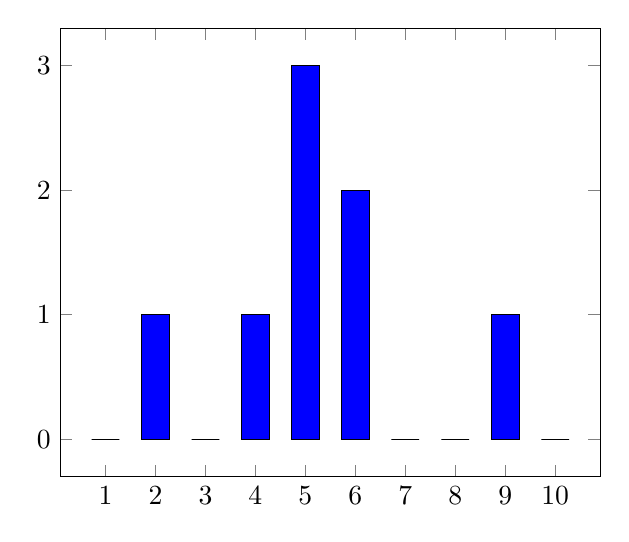
\begin{tikzpicture}
	%\label{bar:results_first}
		\begin{axis}[
			symbolic x coords={1, 2, 3, 4, 5, 6, 7, 8, 9, 10},
			xtick=data
			]
			\addplot[ybar,fill=blue] coordinates {
				(1,  0)
				(2,  1)
				(3,  0)
				(4,  1)
				(5,  3)
				(6,  2)
				(7,  0)
				(8,  0)
				(9,  1)
				(10,  0)
			};
		\end{axis}
	\end{tikzpicture}
\end{figure}

\begin{figure}[!h]
	\centering
	\caption{Fråga 2: Vilken editor har du främst använt för att koda i appen?}
	\begin{tikzpicture}
\pie [text=legend]{100/WebStorm, 0/Annat}
\end{tikzpicture}
\end{figure}

\begin{figure}[!h]
	\centering
	\caption{Fråga 3: Varför valde du denna editor?}
	\begin{tikzpicture}
\pie [text=legend]{25/{Har använt förut, är nöjd}, 37.5/{Någon rekommenderade den, var
bättre än andra allternativ}, 25/{Vet inga andra alternativ som passar}, 12.5/{Annat}}
\end{tikzpicture}
\end{figure}

\begin{figure}[!h]
	\centering
	\caption{Fråga 4: Hur tycker du att ditt val av editor har påverkat utvecklingen av mjukvara? Från ``Försämrat utvecklingen`` till ``Underlättat utvecklingen väldigt mycket``.}
	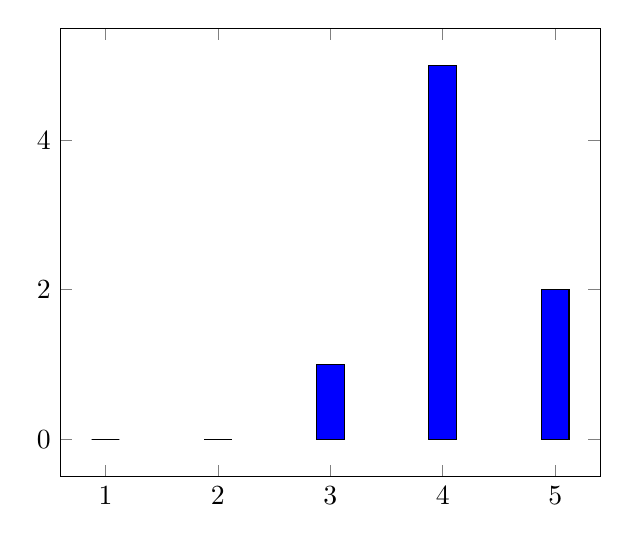
\begin{tikzpicture}
	%\label{bar:results_first}
		\begin{axis}[
			symbolic x coords={1, 2, 3, 4, 5},
			xtick=data
			]
			\addplot[ybar,fill=blue] coordinates {
				(1,  0)
				(2,  0)
				(3,  1)
				(4,  5)
				(5,  2)
			};
		\end{axis}
	\end{tikzpicture}
\end{figure}

\begin{figure}[!h]
	\centering
	\caption{Fråga 5: Hur tycker du att Git har påverkat utvecklingen av mjukvara? Från ``Försämrat utvecklingen`` till ``Underlättat utvecklingen väldigt mycket``.}
	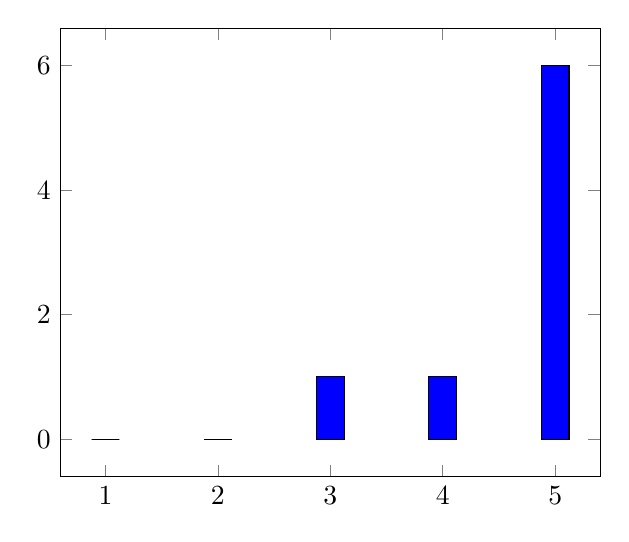
\begin{tikzpicture}
	%\label{bar:results_first}
		\begin{axis}[
			symbolic x coords={1, 2, 3, 4, 5},
			xtick=data
			]
			\addplot[ybar,fill=blue] coordinates {
				(1,  0)
				(2,  0)
				(3,  1)
				(4,  1)
				(5,  6)
			};
		\end{axis}
	\end{tikzpicture}
\end{figure}

\begin{figure}[!h]
	\centering
	\caption{Fråga 6: Har du fått hjälp med Git när du behövt? Från ``Nej`` till ``Alltid``.}
	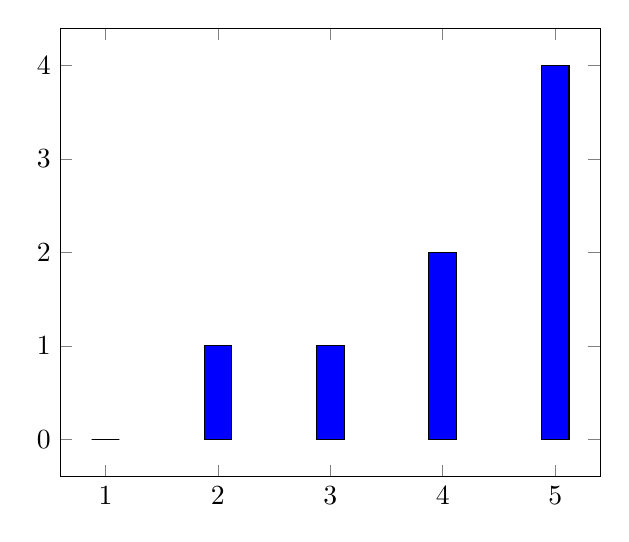
\begin{tikzpicture}
	%\label{bar:results_first}
		\begin{axis}[
			symbolic x coords={1, 2, 3, 4, 5},
			xtick=data
			]
			\addplot[ybar,fill=blue] coordinates {
				(1,  0)
				(2,  1)
				(3,  1)
				(4,  2)
				(5,  4)
			};
		\end{axis}
	\end{tikzpicture}
\end{figure}

\begin{figure}[!h]
	\centering
	\caption{Fråga 7: Hur tycker du att Trello har påverkat utvecklingen av mjukvara? Från ``Försämrat utvecklingen`` till ``Underlättat utvecklingen väldigt mycket``.}
	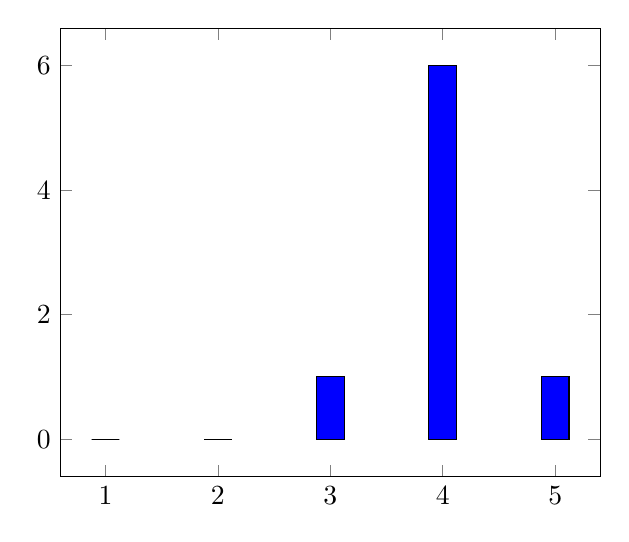
\begin{tikzpicture}
	%\label{bar:results_first}
		\begin{axis}[
			symbolic x coords={1, 2, 3, 4, 5},
			xtick=data
			]
			\addplot[ybar,fill=blue] coordinates {
				(1,  0)
				(2,  0)
				(3,  1)
				(4,  6)
				(5,  1)
			};
		\end{axis}
	\end{tikzpicture}
\end{figure}

\begin{figure}[!h]
	\centering
	\caption{Fråga 8: Hur tycker du att Slack har påverkat utvecklingen av mjukvara? Från ``Försämrat utvecklingen`` till ``Underlättat utvecklingen väldigt mycket``.}
	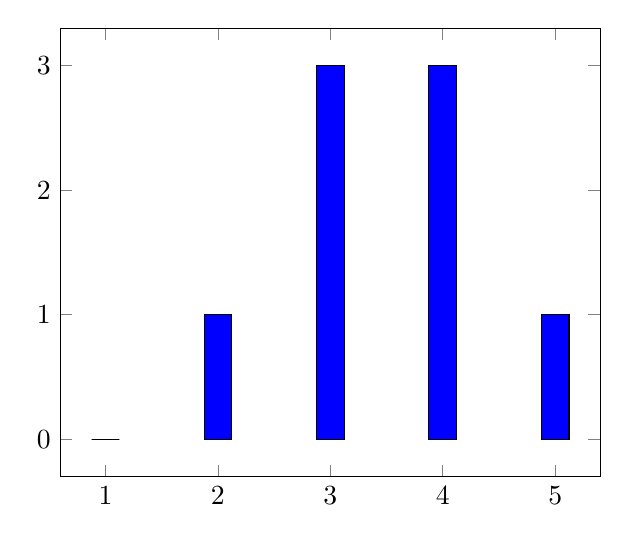
\begin{tikzpicture}
	%\label{bar:results_first}
		\begin{axis}[
			symbolic x coords={1, 2, 3, 4, 5},
			xtick=data
			]
			\addplot[ybar,fill=blue] coordinates {
				(1,  0)
				(2,  1)
				(3,  3)
				(4,  3)
				(5,  1)
			};
		\end{axis}
	\end{tikzpicture}
\end{figure}

\begin{table}[h!]
\centering
  \caption{Fråga 9: Vilka problem ser du med de verktyg vi använt för att utveckla mjukvara?}
  \def\arraystretch{1.5}
  \begin{adjustbox}{max width=\textwidth}
    \begin{tabularx}{\textwidth}{| X |}
      \hline
      \textbf{Svar} \\
      \hline
      Ibland saknas det kompetens för att utnyttja verktyget till fullo \\
      \hline
      Inga direkta problem. \\
      \hline
      Har svårt att se problem då jag inte har bra koll på många andra alternativ. Förutom det så har jag inte upplevt några problem.\\
      \hline 
      Ser inga problem med dem\\
      \hline 
      Dålig disciplin/konventioner i Slack och Trello leder till oordning \\
      \hline 
      Git: Viss inlärningströskel. Webstorm: aningen resurskrävande på laptop. Slack: Mycket meddelanden, som man inte alltid läser och därför kanske missar något viktigt. Trello: Inga problem.\\
      \hline 
      Verkar vara en stabil editor\\
      \hline  
      Inga, är bekväm med allt.\\
      \hline
    \end{tabularx}
  \end{adjustbox}
\end{table}

\begin{table}[h!]
\centering
  \caption{Fråga 10: Vilka problem ser du med hur verktygen har använts av gruppmedlemmarna?}
  \def\arraystretch{1.5}
  \begin{adjustbox}{max width=\textwidth}
    \begin{tabularx}{\textwidth}{| X |}
      \hline
      \textbf{Svar} \\
      \hline
      Man har använd verktygen olika och detta kan ha lätt till förvirring, tillexempel kommentarer på trellokort \\
      \hline
      Alla har inte varit på samma nivå med tex Git och vissa har inte brytt sig om att följa de regler vi satt upp. \\
      \hline
      Varierande kunskap har definitivt påverkat hur folk använder verktygen, det kan ibland ha satt käppar i hjulen men inget allvarligt så det är svårt att specificera.\\
      \hline 
      Vissa har inte lärt sig git tillräckligt bra\\
      \hline 
      Gruppmedlemmar skulle behöva mer kompetens inom verktygen så att ingen skriver t.ex. "git rm .". \\
      \hline 
      Inget egentligen\\
      \hline 
      Inget man reflekterat över, man bara kör på\\
      \hline  
      Git add . Skulle kunna ha haft nån kort genomgång hur man gör.\\
      \hline
    \end{tabularx}
  \end{adjustbox}
\end{table}

\begin{table}[h!]
\centering
  \caption{Fråga 11: Om du skulle vilja ändra något med verktygen eller hur de används, vad skulle det vara?}
  \def\arraystretch{1.5}
  \begin{adjustbox}{max width=\textwidth}
    \begin{tabularx}{\textwidth}{| X |}
      \hline
      \textbf{Svar} \\
      \hline
      Inbyggda videokonferenser i Slack. Prioriteringsbara kort i Trello. \\
      \hline
      Att hålla mer fokuserade diskussioner i Trello-kort istället för en Slack-chatt hade gjort problem i utvecklingen lättare att följa. \\
      \hline
      Ingenting\\
      \hline 
      Svårt att veta när man inte har jobbat i en annan editor för webbprogrammering tidigare så man kan inte jämnföra.\\
      \hline 
    \end{tabularx}
  \end{adjustbox}
\end{table}

\begin{table}[h!]
\centering
  \caption{Fråga 12: Om du kan, hitta på ett verktyg som vi skulle kunna använda för att ytterligare underlätta för utvecklingen av mjukvara i vår grupp.}
  \def\arraystretch{1.5}
  \begin{adjustbox}{max width=\textwidth}
    \begin{tabularx}{\textwidth}{| X |}
      \hline
      \textbf{Svar} \\
      \hline
      Ett övergripande planeringsverktyg för att tydligt se flödesschema på vilka uppgifter som bygger på varandra och i vilken ordning saker behöver göras. Trello saknar den biten. \\
      \hline
      Ett system där en process som kräver validering och testning innan kod kan pushas hade varit användbart för att säkerställa kvalitet. Gärna integrerat (eller med tillhörande) Trello-funktionalitet för att spåra arbetet \\
      \hline
      en voice-to-text så man slipper använda händerna.\\
      \hline 
    \end{tabularx}
  \end{adjustbox}
\end{table}